\documentclass[12pt]{article}
\usepackage{hyperref}
\usepackage{graphicx}
\graphicspath{{./}}
\usepackage{dirtytalk}
\usepackage{listings}
\lstset{basicstyle=\small\ttfamily,
    columns=flexible,
    breaklines=true
}


\title{Implementing Security Rules, Safeguards, and IDS tools for Private Cloud Infrastructures}
\author{Author: Aleksander Okonski -- aleksander.oko@gmail.com \\ Supervisor: Salman Toor \\ Review: Bjorn Victor }
\date{}


\begin{document}
\maketitle
\newpage
\tableofcontents
\newpage

\section{Background}
The cloud computing space has grown over the last several years. Business and Universities are looking at solutions to migrate their existing infrastructure to the cloud. There are several reasons for this type of business shift: costs, scalability, reliability \cite{DillonWuChang}. The cloud offers some precedented advantages to a standardized computational model. One is able to pay for only the resources used, with more resources added/removed depending on the demand. Another advantage is the ability to spine up/destroy several machines with little overhead. Several companies are fronting the cloud revolution including Amazon, Google, Microsoft, and Digital Ocean. These companies are providing a public cloud environment, that is to say that anyone can pay for computer resources. Other companies such as RackSpace, IBM, and VMware are providing private / hybrid cloud resources.

\subsection{Cloud Models}
As mentioned above the cloud space consists of three types of clouds: public, hybrid, and private. The public cloud enables anyone to connect to the host and set up a machine. The host machines that run the cloud environment are located in public data centers throughout the world. The virtual machines are created then run and can be connected to the Internet.  The private cloud consist of the host being located in a private hosting environment. The virtual machines that are created are collocated on the internal network. The hybrid environment merges the two, with having some of the machines collocated in private data centers and others located on public data centers. Each of these models have benefits and drawbacks and have to evaluated for each individual project. The these cloud models all share a smilier set of tools employed to provide the necessary computational recourses to users.

In the cloud computing space several computational models exist \cite{wikipedia}. These models reflect the different stages of a computer: hardware (Software as a Service), operating system (Platform as a Service), and software (Software as a Service).

\begin{itemize}
    \item Software as a Service (SaaS) allows for the user to utilize applications (I.E. Email, games, etc.) without the need to set up / worry about the underlying infrastructure. The cloud provider would be responsible with ensuring that the infrastructure and OS are running correctly.
    \item Platform as a Service (PaaS) give the user the ability to create applications (I.E. Web servers, databases, etc.) without the need to create the entire system from the ground up.
    \item Infrastructure as a Service (IaaS) gives the users a basic virtual machine with the user needing to set up all necessary functionality. This moves the responsibility of management of the hardware, network, and storage from the user to the operator.
\end{itemize}

\subsection{Cloud Infrastructure}
At the most fundamental layer a cloud computer is a server running in a data-center that has a hypervisor which then contains and runs another operating system. These hypervisores are the backbone of cloud computing allowing several virtual environments to use the same hardware. A hypervisor is a layer of code that sits between the computer components (bare metal) and the guest OS\@. The hypervisor then translates instructions from the guest system onto the hardware. There are several different hypervisors to choose from (Xen, Oracle VirtualBox, Oracle VM, KVM, VMware ESX/ESXi, or Hyper-V) with each having similar outcomes through different approach to the problem. To control the users and virtual machines many cloud providers (Amazon, Google, etc.) have created proprietary solutions. However, NASA and RackSpace Hosting \cite{wikipedia1} have created an open source version called OpenStack.

\subsection{Cloud Roles}
When cloud computing first started to take off, the main type of computing resource provided was IaaS in the public cloud \cite{sourcedigit}. This started to change in the recent years when two new types models for cloud computing emerged. Public and Hybrid clouds allowed for companies to utilize the power of the cloud while still having some or all of there resources located in their own data centers.

\subsection{Cloud Computing vs Standard Models}
Cloud computing has some distinct differences from regular computing. The systems are

\begin{itemize}
    \item Systems do not usually stay active for long. Users will provision and destroy systems with a high turnover.
    \item Users may spin up several machines at once.
    \item There may not be a dedicated team used to ensure up time / health of systems.
    \item Users will usually have full control of the systems.
\end{itemize}

Cloud computing also has a different threat model compared to a normal dedicated server \cite{zissis2012addressing, mishra2013cloud, krutz2010cloud}. With normal server infrastructure the infrastructure and system are built once and then ran for extended periods of time. The systems themselves are not refreshed or rebuilt as happens in the cloud.

\section{Related Work}
In this work we will be looking at ways to protect VM clusters by ensuring proper configuration steps are setup and used with the addition of looking at ways to implement an IDS solution into the cloud environment. Before starting the work, we looked into previous work done in this field. Cloud security had been a hot topic in recent times therefor several papers have been written \cite{zissis2012addressing, mishra2013cloud, krutz2010cloud}. These particular papers focus on the different aspects and concerns that are present when running in a cloud environment. They are a nice starting point to look at how the threat landscape in the cloud differs from the slandered model. An important distinction of how information is treated differently in a centralized and cloud environments is talked about in "Assessing Cloud Computer Security Issues" \cite{zissis2012addressing}. The three staples of information security are confidentiality, integrity, and availability. In the cloud new difficulties come up for each of these classifications as data in the cloud is now accessible to more individuals.  The second set of articles looked at was about intrusion detection systems (IDS), more specifically how these can be used within the cloud \cite{SurveyOfIDS, patel2013intrusion}. These articles did not focus so much on implementation as they were focused more on the theory. An interesting comparison that shows the advantages and disadvantages for different IDS systems is table $2$ in \cite[SurveyOfIDS]. This is the basis for the types of IDS solutions that were chosen for this project. As this work was primarily focused on OpenStack, one particular IDS conference talk was used as a starting point for this research \cite{videoPresentation}.

%expand more on related work with writing some things in my own words and then refering back to the articals.
%i have arcitected this in such a way beocuse i read this and that
%Connect your work with the other projects and tell how they are diffrent!

\section{OpenStack}
OpenStack is an open source platform for cloud computing \cite{wiki:OpenStack}. OpenStack is built of many components that are designed to provide a different set of services (Nova, Neutron, etc.) the full list can be found on the open stack website located \href{https://www.openstack.org/software/project-navigator/}{here}. OpenStack is very scalable and diverse system that can be arranged to fit the needs of any cloud environment. For this project we ran OpenStack newton version 15.0.0.0.rc1. OpenStack is very modular with several core features running as the backbone of the software. The features that were used for this project were: Nova, Neutron, and Swift.

Nova is the platform that provides access to OpenStack compute resources. It is the base platform that a user would interact with the set up, run, configure, and destroy machines. Neutron is the service that controls and configures all of the networking between machines and the external network. Swift is the platform that is used for object and blob storage.


%What relsea, functionalities
%This projec thas a core interest in nova, etc.

%section comprehensive aobu security in the cloud
%Terms related to cloud security (what is IDS)
% what are the main streams in security
% introduction to network security
\section{Security}
The field of computer security is large and diverse \cite{ComputerSecurity}. The general focus of computer security is to ensure that computer systems follow the CIA model of confidentiality, integrity, and availability. "The design artifacts that describe how the security controls (security countermeasures) are positioned, and how they relate to the overall IT Architecture. These controls serve the purpose to maintain the system's quality attributes, among them confidentiality, integrity, availability, accountability and assurance." \cite{it_security_architecture} The disciplines that are focused on in this paper include: intrusion detection systems, network security, and system security.
Intrusion detection systems come in two main forms, host based and network based. A host based system runs on the host and attempts to detect any security threats on the host machine. A network based IDS is connected on the network and inspects network traffic, trying to find threats by inspecting network traffic patterns. Both of these systems have advantages and disadvantages. With a host based system software must be installed and configured on each system. In a network IDS system the packets are monitored for unusual traffic patterns. There are disadvantages to this type of solution also, mainly network traffic can be encrypted and the overall volume of traffic encountered. Some examples of network based IDS tools are \href{https://www.snort.org/}{Snort}.
A large portion of the problem for computer security comes from the networks that computers are attached to. The network allows other computers to communicate and attempt to access the particular machine. This is greatly increased if the computer is not placed behind a firewall/rougher and is directly accessible form the Internet. If an Internet facing computer is not updated properly vulnerabilities can be used to run unintended programs.
A unintended program running on a systems can be a concern due to several. These programs can be used to send email spam, steal credentials, or participate in larger network attacks.

%For a cloud system where machines are provisioned and destroy setting up this type of system would be difficult. There for a network based IDS system was chosen.

\section{User Recommendation}
The first stage of this project involved setting up user recommendations for configuring a secure VM and understanding some security features in the OpenStack platform.

\section{Design Implementation}
For the first part of the project a modular design was created to enable further types of scanning to be added. An important aspect when designing the watchdog system with as little privileges as possible to prevent any unnecessary security holes. The following is a diagram of an example cloud environment.
\\
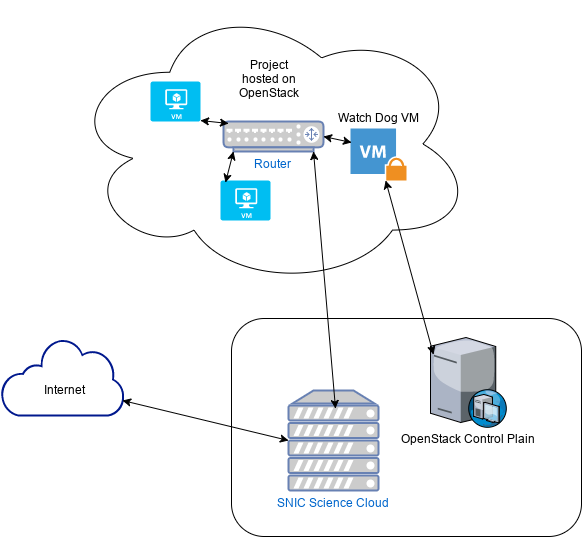
\includegraphics[scale=.3]{./pic/flowchart.png}
\\
The "watchdog" is initiated in the cloud cluster. The once initiated the VM will connect to the OpneStack Control Plain and get the list of servers, IP's, and floating IP's. Once that information is retreated the different modules will be run. In this standard case the two modules created were for nmap and ssh\_scan. Nmap is a tool used to scan a local or external network nd view what machines are funning on it. Nmap will be able to scan the machines ports and tell which ones are open and what services are running on them. It will also try and guess heuristically the operating system that is being run on the machine. This tool is therefor used in this system to find machines that have open ports and to see what services are run on them. If a service or port is found to not follow the recommendation then the machines can be terminated. The ssh\_scan tool is used to ensure that only a public private key pair are used. It will scan port 22 and alert if any other form of authentication is used.
These modules will gather the results from the network and collect them into a central repository. Once the data is gathered it is compared to the config file.  If a discrepancy is found between the expected results and the scanned machine is found an alert is sent to the administrator. For this project the administrator receives notification on a separate slack. This entire process is run every 20 min by a corn job located on the watchdog machine. This type of design allows for a flexible platform that can have each component further customized.

A key part of this project was to create a simplistic interface that would allow an administrator to view changes to the environment and query for more information. Some base goals were created: scalability, ease of use, and intuitiveness. As the system is designed to be deployed over several cloud groups we needed a messaging system that could handle such a task. Email was first considered however it was soon realized that email would not work well due to the frequency of data sent and then inability to interact with the service. The next consideration was Internet Relay Chat (IRC), however as IRC is relatively unused in the professional work environment and users would need to learn how to interact with the protocol that idea was abandoned. Therefor as a final solution it was decided to work to build the messaging solution using Slack. This matched all of our starting criteria and allowed for a clean and simple implementation. Slack is a messaging application that allows groups of users to interact with one another in channels or directly. Once of the really neat features of this is the ability to program bots for users to interact with. Therefor the decision was made to create a bot that would interact with a channel for each cluster of machines. The bot would update the channel with any new information that the scan found ensuring that a constant flow was preserved. Users are also able to query to bot directly and get more information about the environment. This allows seamless integration between getting information from the environment and being able to dive deeper and investigate a machine.



\section{Architecture}

tmp

%part 2 look if the router can be accesed to pull network stream
% gather memory print / services / programs / work load


\newpage
\bibliographystyle{plain}
\bibliography{thesis.bib}
\end{document}
